\begin{frame}
	\frametitle{Test Plot 1}
	\begin{figure}%
	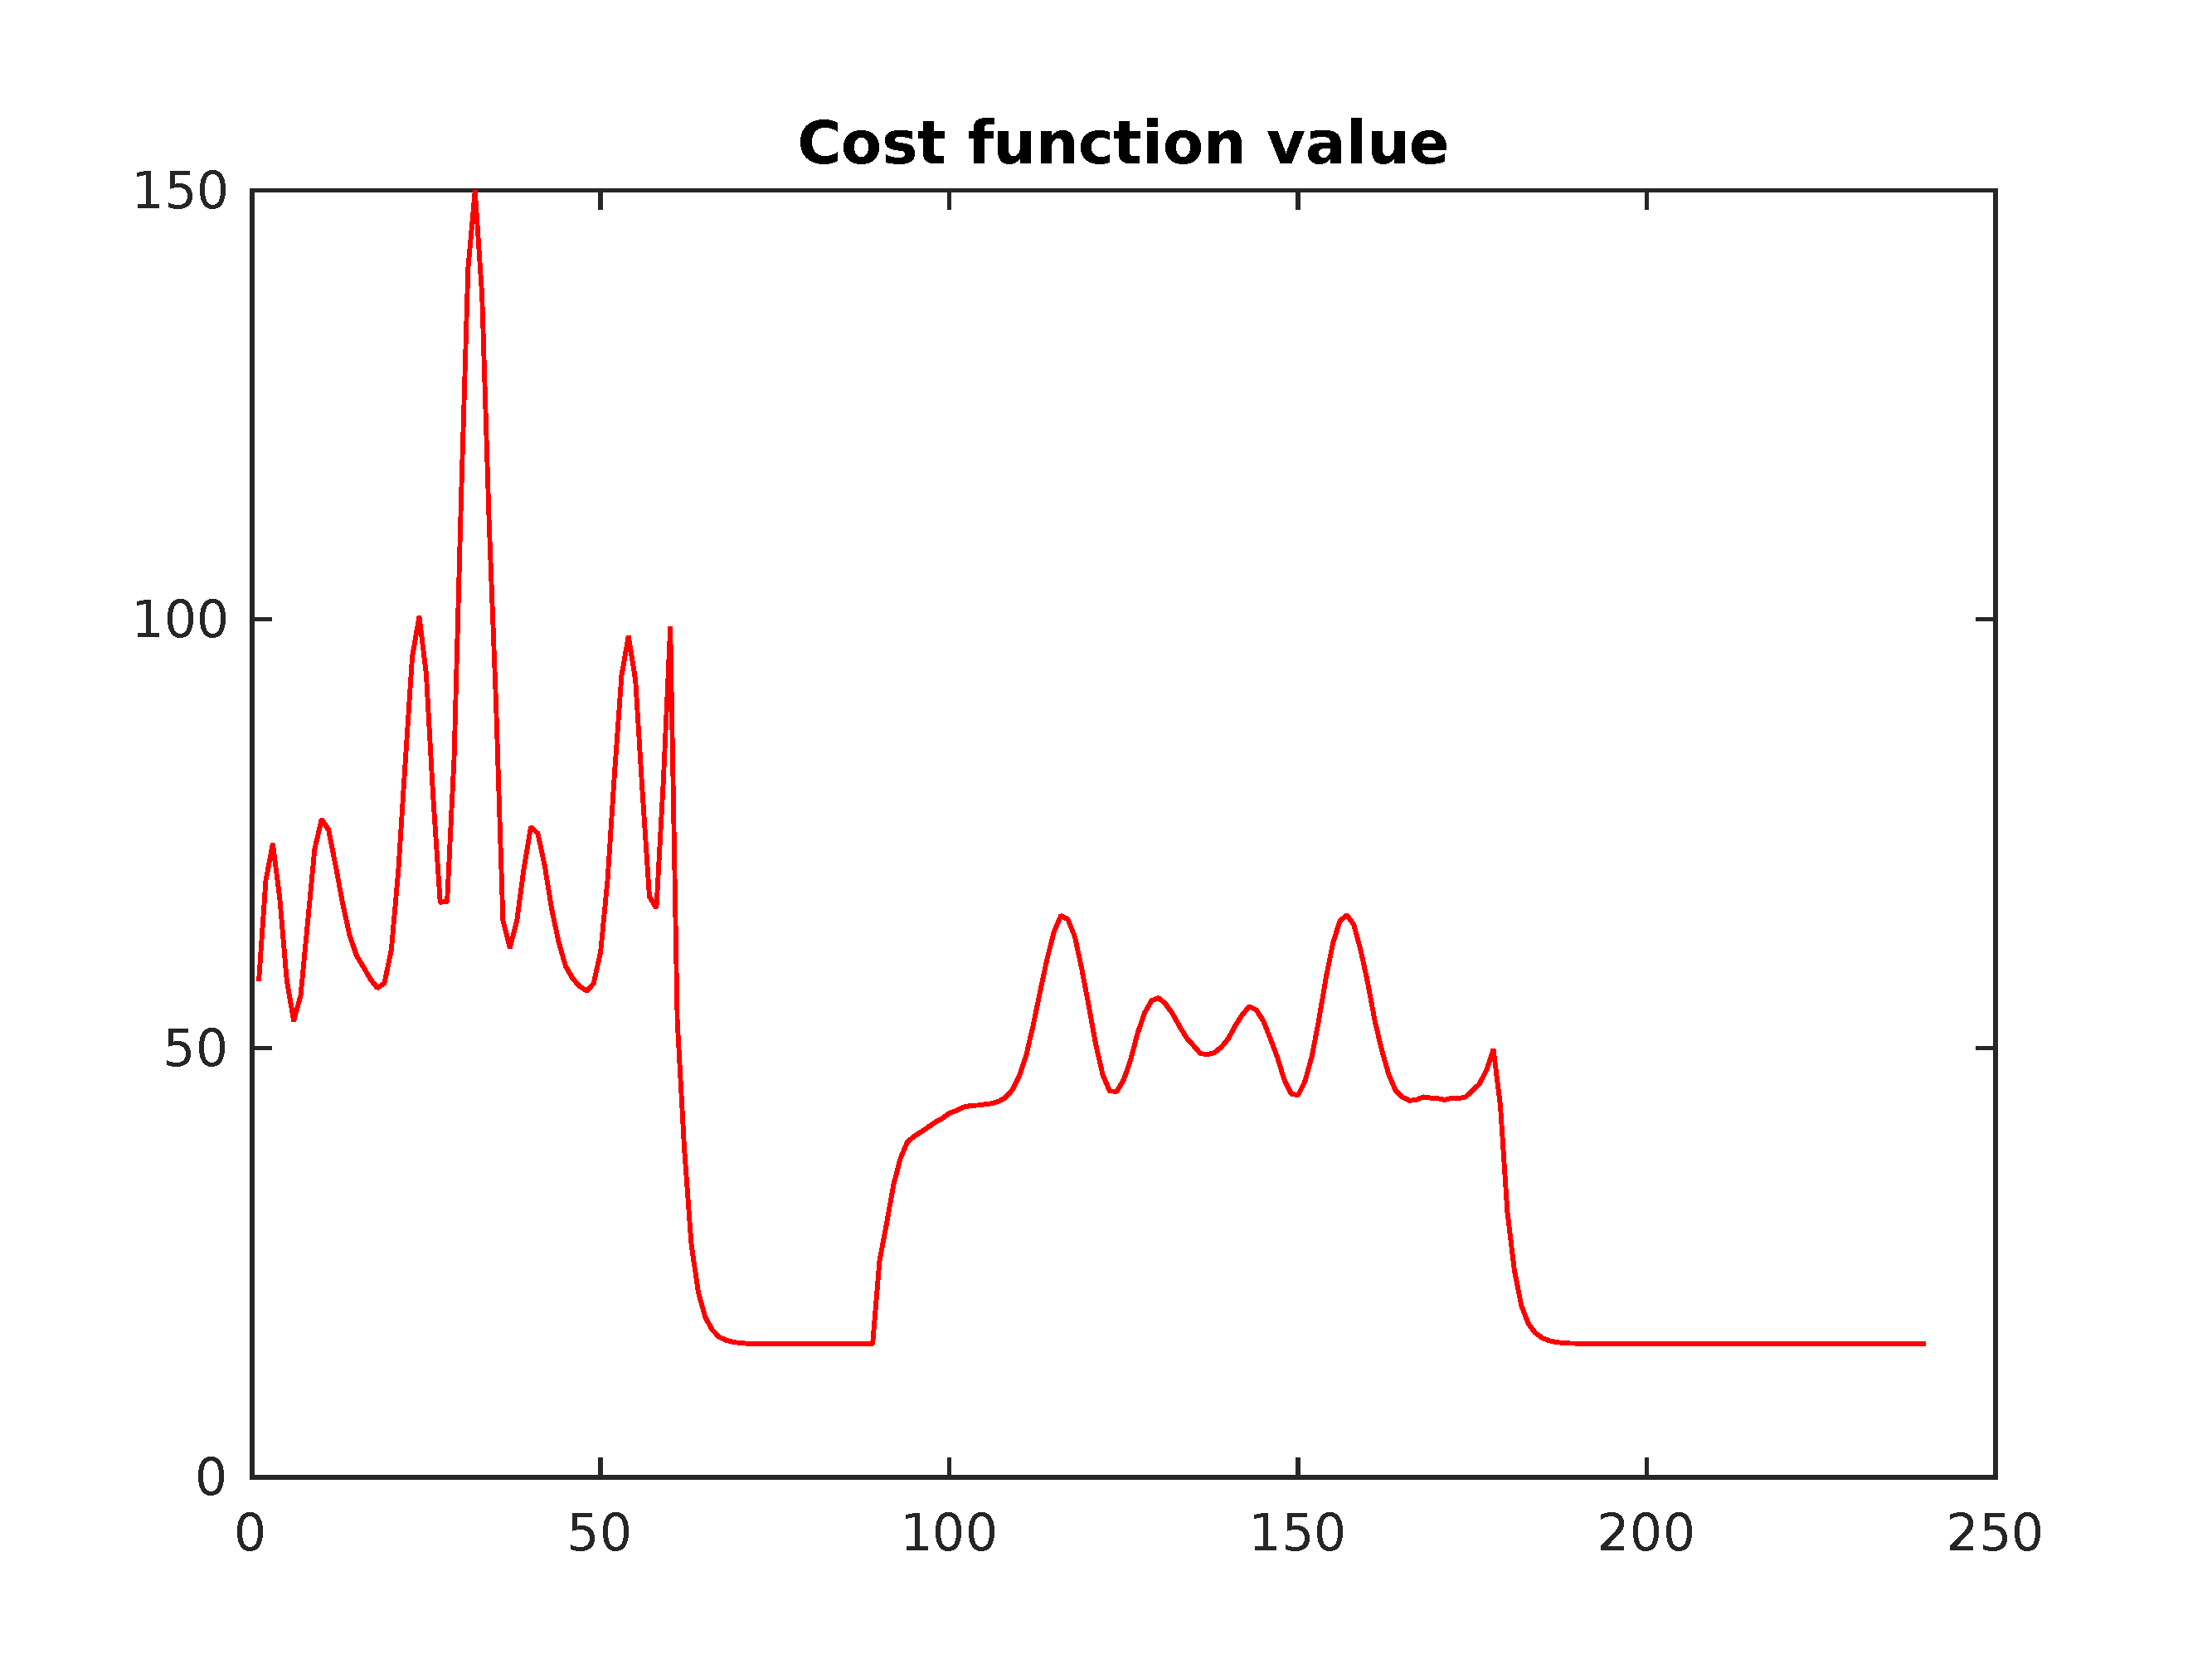
\includegraphics[width=0.75\columnwidth]{images/costF}%
	\caption{unser erster toller Plot}
	\end{figure}
\end{frame}

\begin{frame}
	\frametitle{Test Plot 1}
	\begin{figure}%
	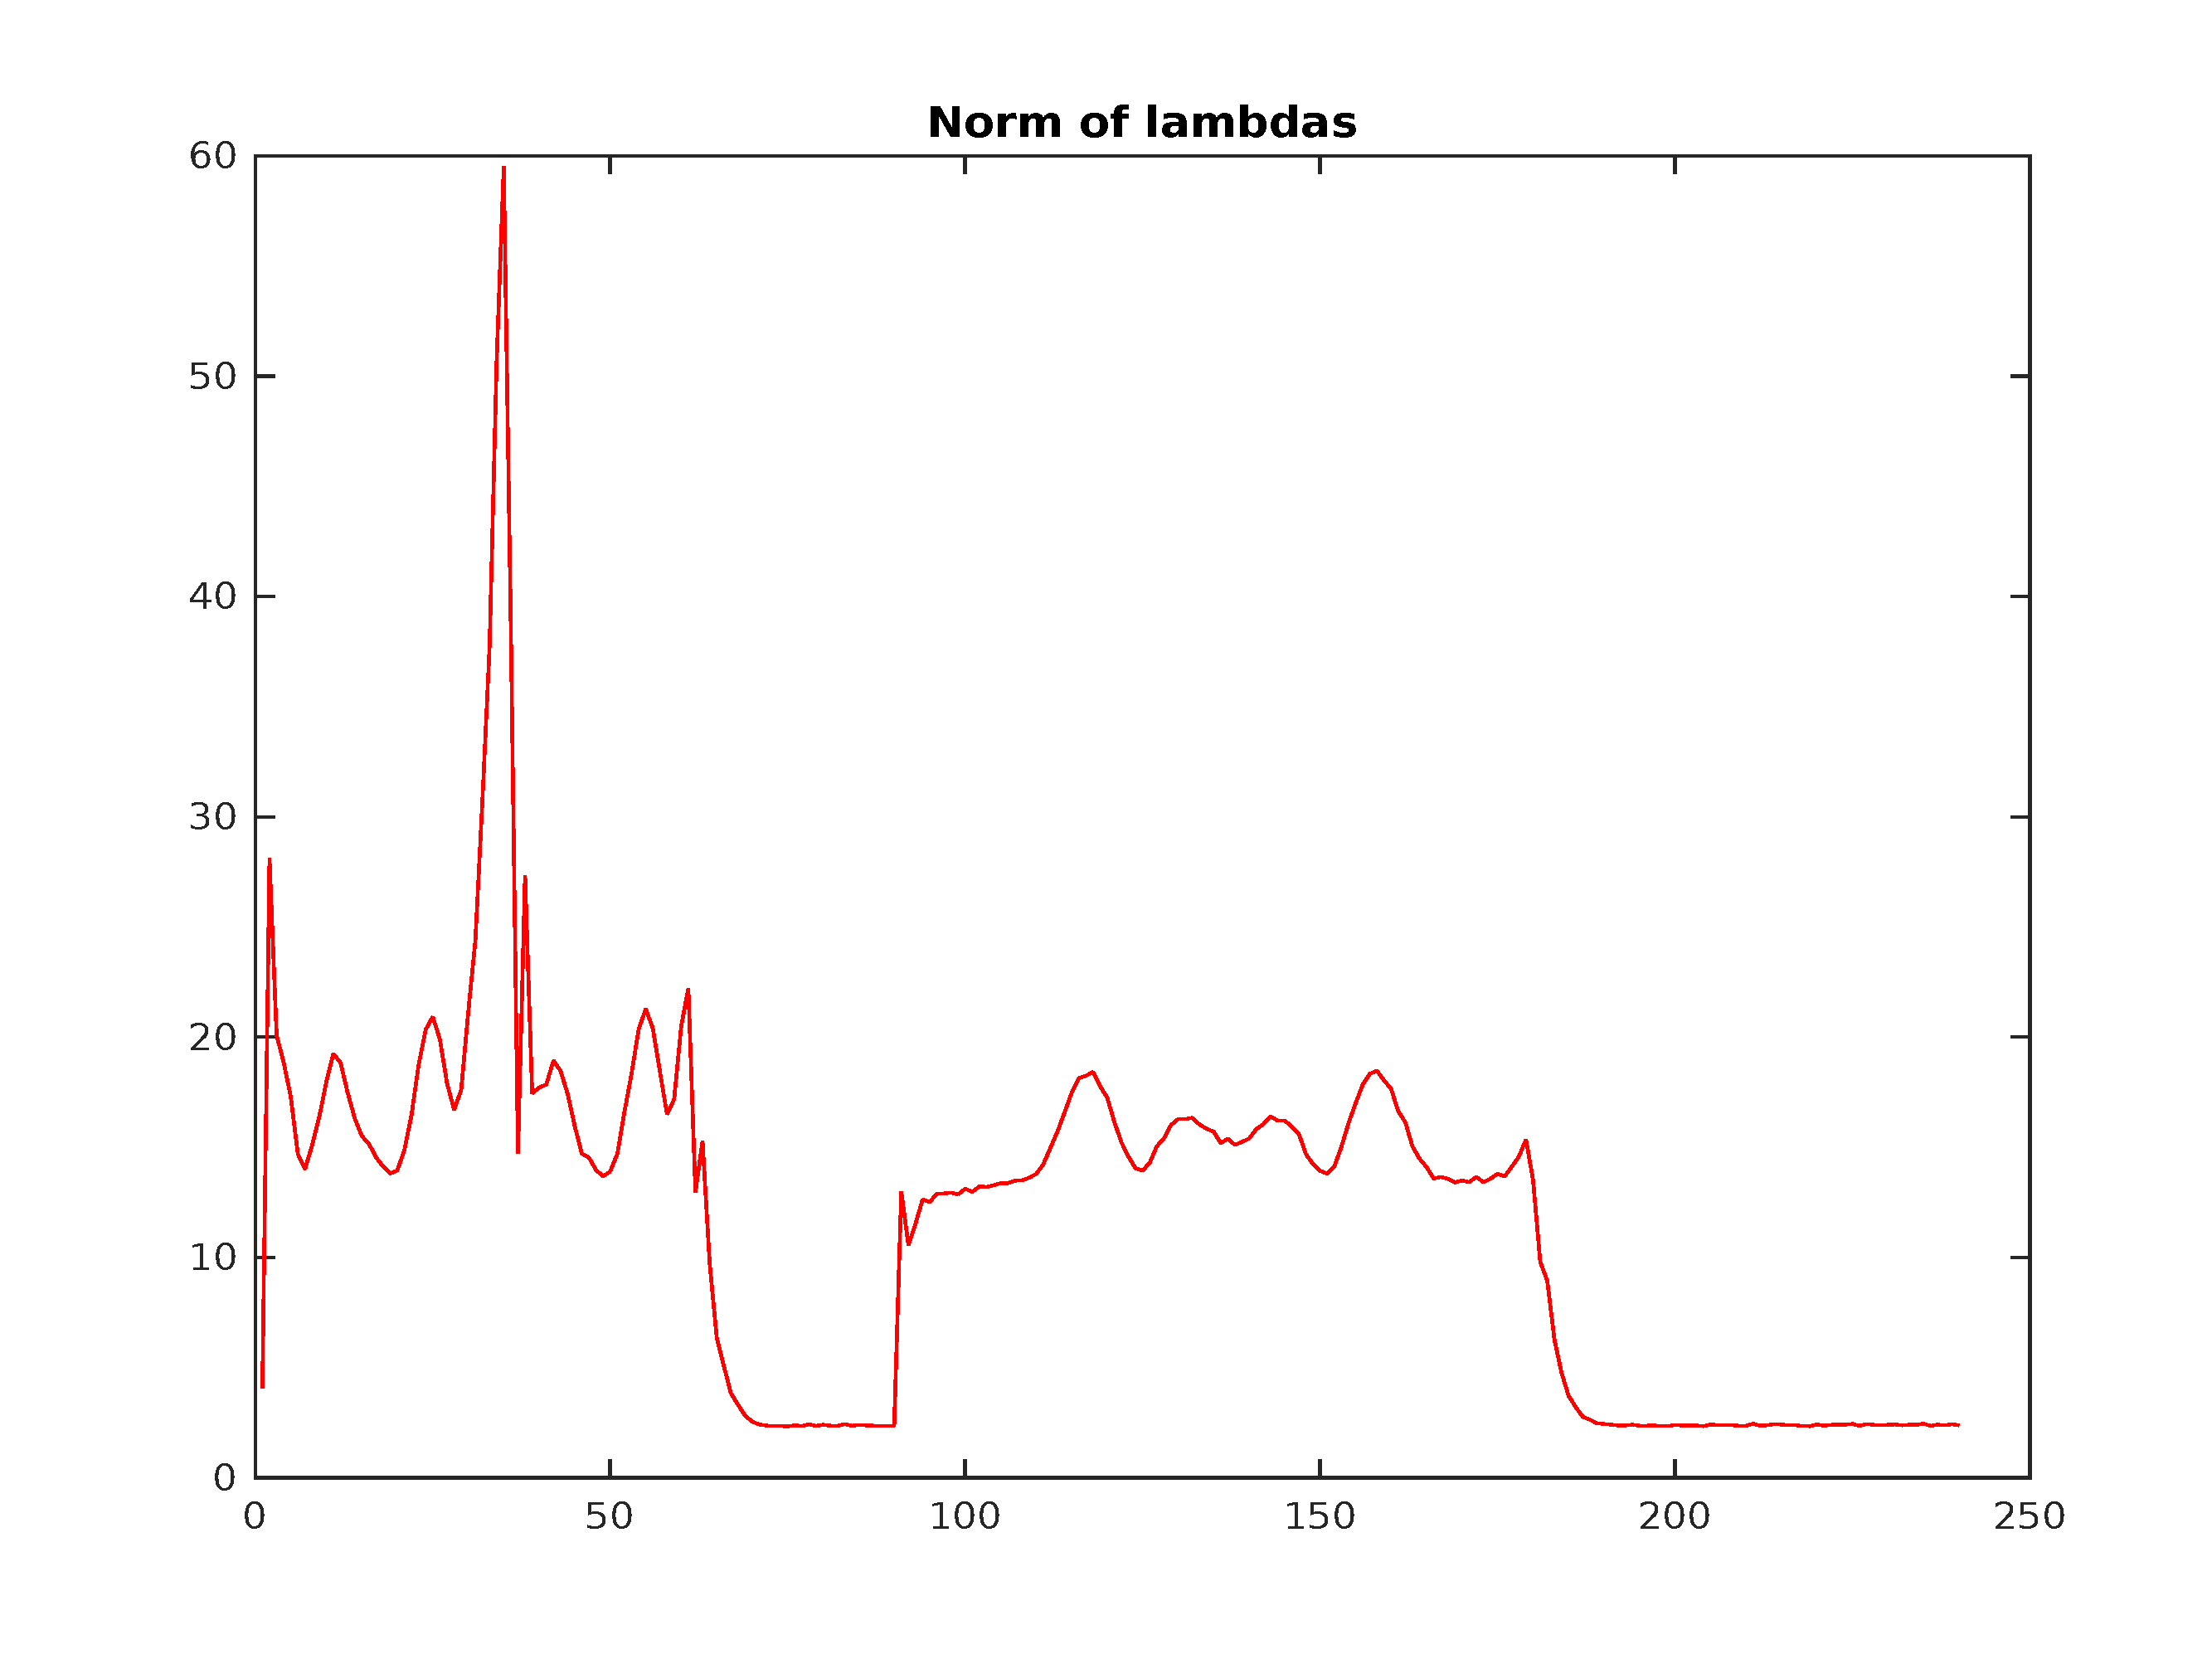
\includegraphics[width=0.75\columnwidth]{images/norm_lambda}%
	\caption{unser erster toller Plot}
	\end{figure}
\end{frame}

\begin{frame}
	\frametitle{Test Plot 1}
	\begin{figure}%
	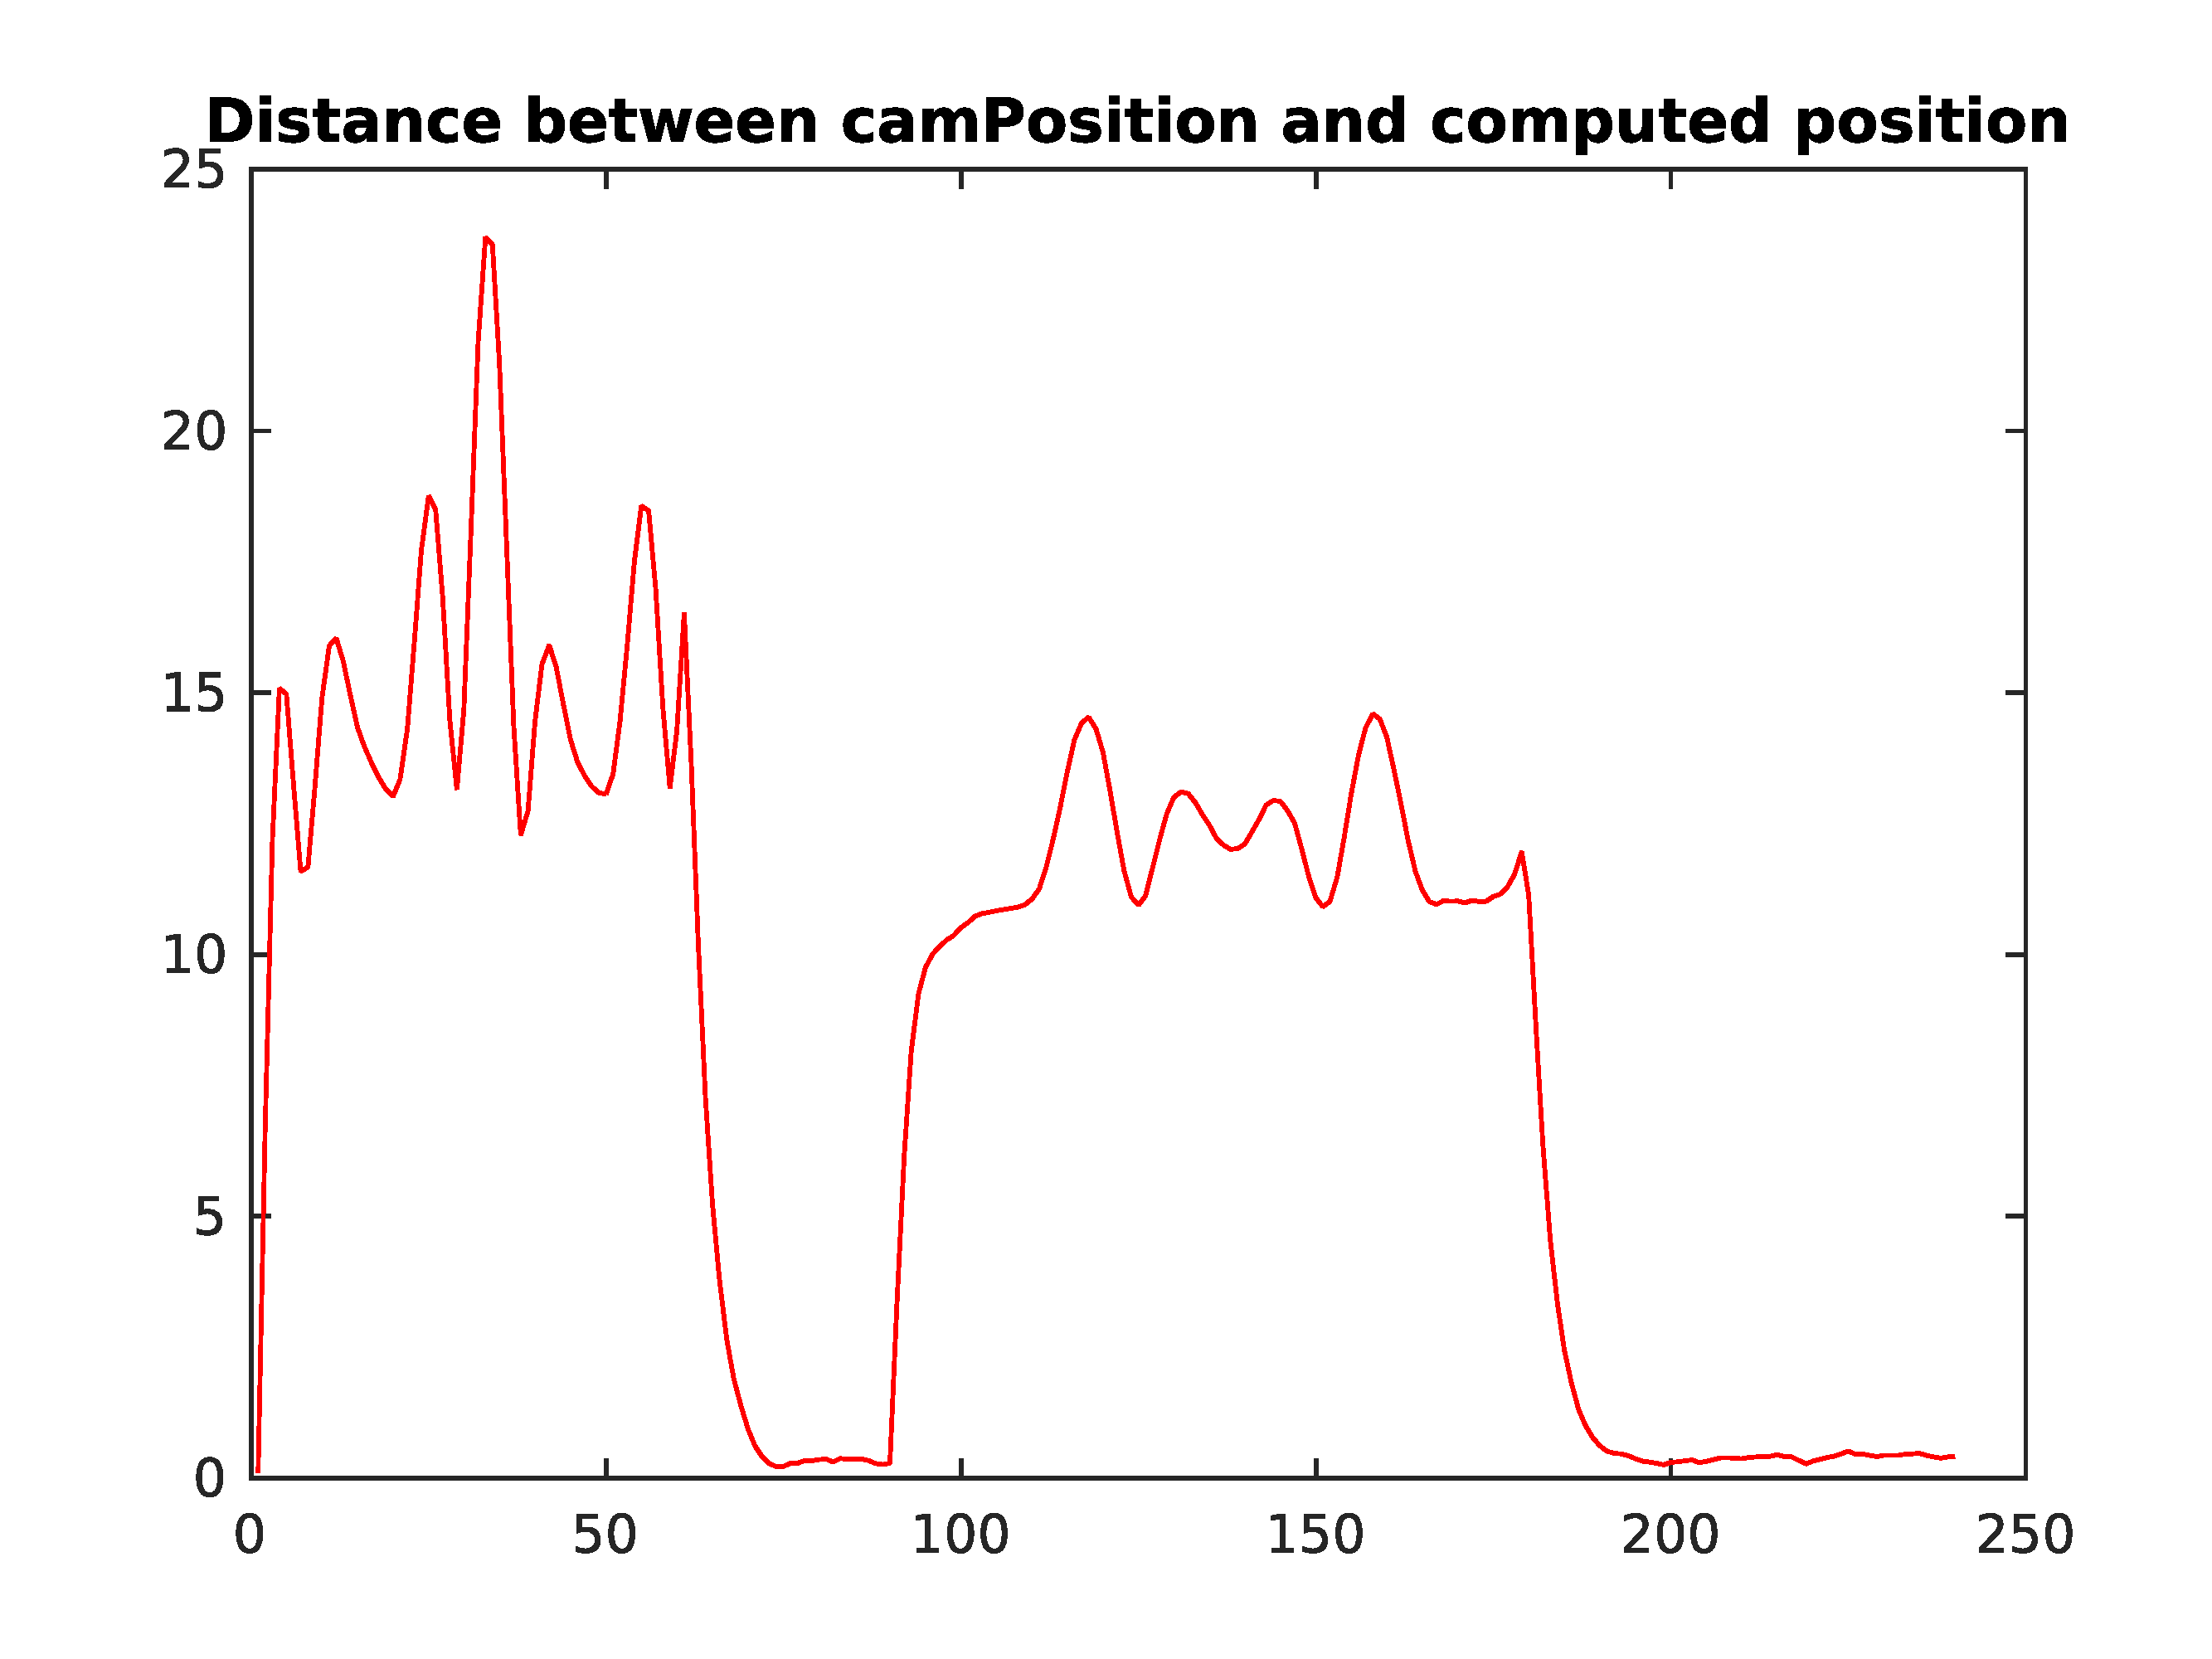
\includegraphics[width=0.75\columnwidth]{images/norm_t}%
	\caption{unser erster toller Plot}
	\end{figure}
\end{frame}

\begin{frame}
	\frametitle{Test Plot 1}
	\begin{figure}%
	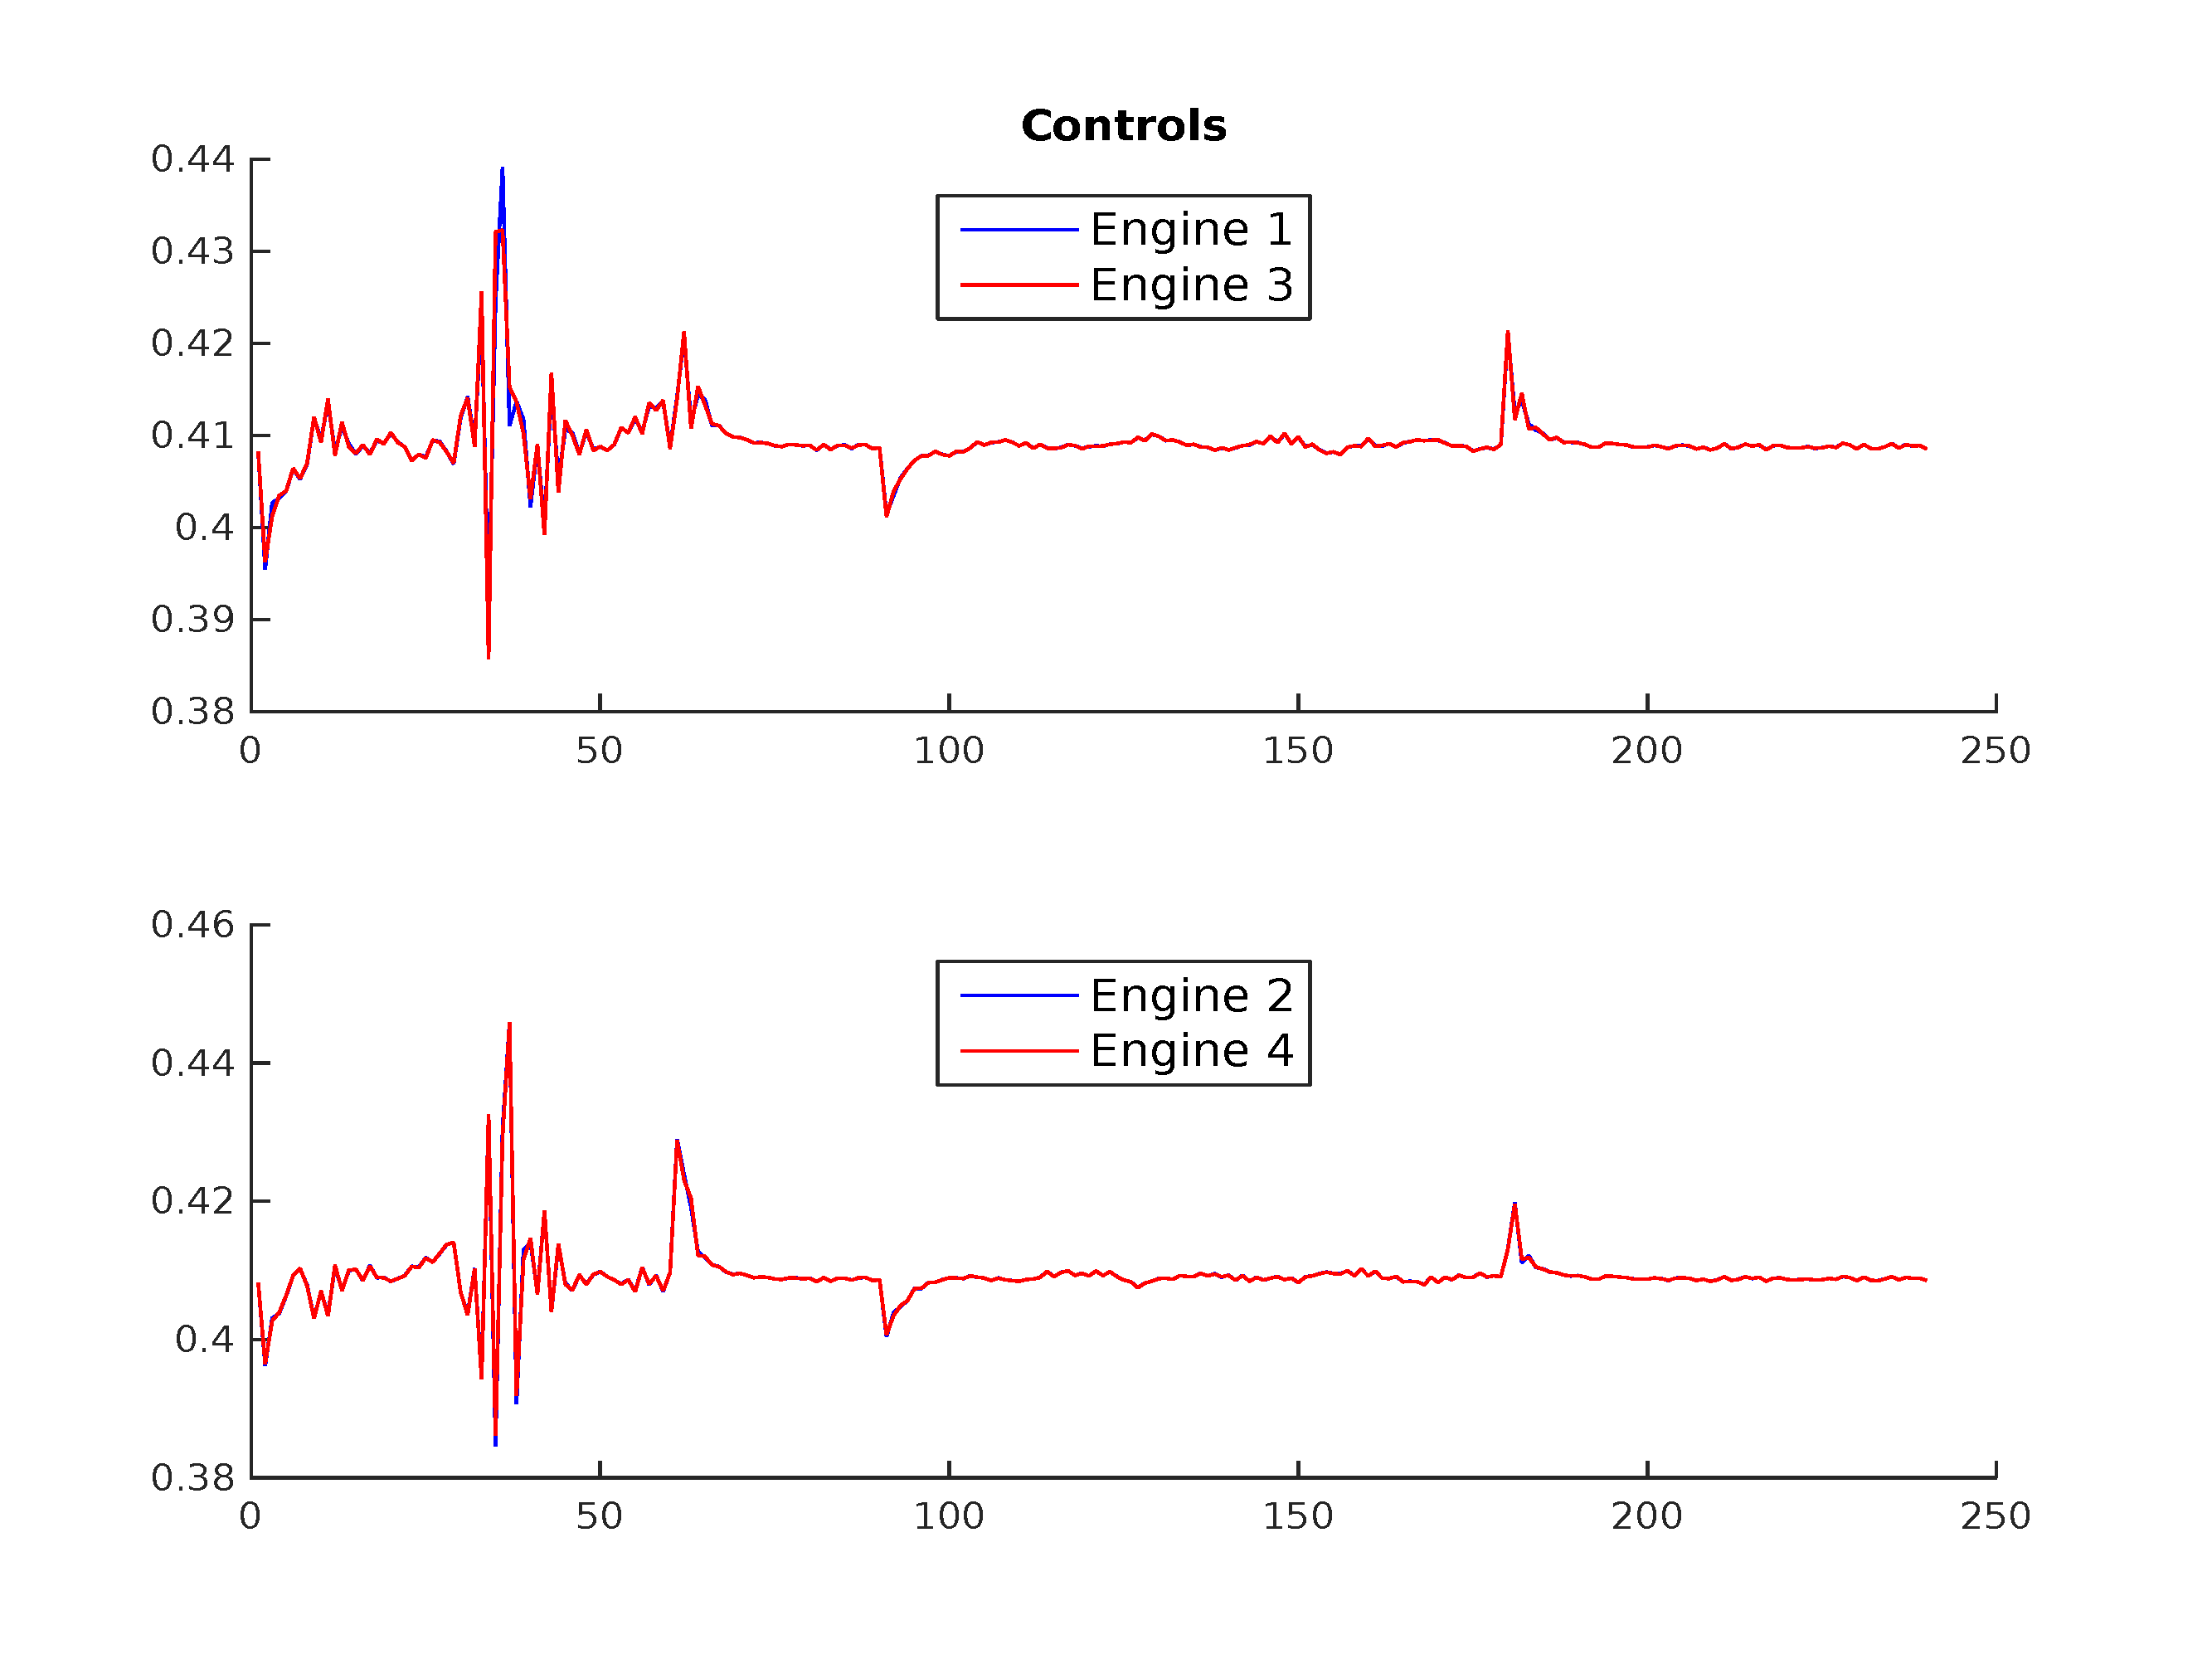
\includegraphics[width=0.75\columnwidth]{images/controls}%
	\caption{unser erster toller Plot}
	\end{figure}
\end{frame}